% Options for packages loaded elsewhere
\PassOptionsToPackage{unicode}{hyperref}
\PassOptionsToPackage{hyphens}{url}
%
\documentclass[
]{article}
\usepackage{amsmath,amssymb}
\usepackage{lmodern}
\usepackage{iftex}
\ifPDFTeX
  \usepackage[T1]{fontenc}
  \usepackage[utf8]{inputenc}
  \usepackage{textcomp} % provide euro and other symbols
\else % if luatex or xetex
  \usepackage{unicode-math}
  \defaultfontfeatures{Scale=MatchLowercase}
  \defaultfontfeatures[\rmfamily]{Ligatures=TeX,Scale=1}
\fi
% Use upquote if available, for straight quotes in verbatim environments
\IfFileExists{upquote.sty}{\usepackage{upquote}}{}
\IfFileExists{microtype.sty}{% use microtype if available
  \usepackage[]{microtype}
  \UseMicrotypeSet[protrusion]{basicmath} % disable protrusion for tt fonts
}{}
\makeatletter
\@ifundefined{KOMAClassName}{% if non-KOMA class
  \IfFileExists{parskip.sty}{%
    \usepackage{parskip}
  }{% else
    \setlength{\parindent}{0pt}
    \setlength{\parskip}{6pt plus 2pt minus 1pt}}
}{% if KOMA class
  \KOMAoptions{parskip=half}}
\makeatother
\usepackage{xcolor}
\usepackage[margin=1in]{geometry}
\usepackage{color}
\usepackage{fancyvrb}
\newcommand{\VerbBar}{|}
\newcommand{\VERB}{\Verb[commandchars=\\\{\}]}
\DefineVerbatimEnvironment{Highlighting}{Verbatim}{commandchars=\\\{\}}
% Add ',fontsize=\small' for more characters per line
\usepackage{framed}
\definecolor{shadecolor}{RGB}{248,248,248}
\newenvironment{Shaded}{\begin{snugshade}}{\end{snugshade}}
\newcommand{\AlertTok}[1]{\textcolor[rgb]{0.94,0.16,0.16}{#1}}
\newcommand{\AnnotationTok}[1]{\textcolor[rgb]{0.56,0.35,0.01}{\textbf{\textit{#1}}}}
\newcommand{\AttributeTok}[1]{\textcolor[rgb]{0.77,0.63,0.00}{#1}}
\newcommand{\BaseNTok}[1]{\textcolor[rgb]{0.00,0.00,0.81}{#1}}
\newcommand{\BuiltInTok}[1]{#1}
\newcommand{\CharTok}[1]{\textcolor[rgb]{0.31,0.60,0.02}{#1}}
\newcommand{\CommentTok}[1]{\textcolor[rgb]{0.56,0.35,0.01}{\textit{#1}}}
\newcommand{\CommentVarTok}[1]{\textcolor[rgb]{0.56,0.35,0.01}{\textbf{\textit{#1}}}}
\newcommand{\ConstantTok}[1]{\textcolor[rgb]{0.00,0.00,0.00}{#1}}
\newcommand{\ControlFlowTok}[1]{\textcolor[rgb]{0.13,0.29,0.53}{\textbf{#1}}}
\newcommand{\DataTypeTok}[1]{\textcolor[rgb]{0.13,0.29,0.53}{#1}}
\newcommand{\DecValTok}[1]{\textcolor[rgb]{0.00,0.00,0.81}{#1}}
\newcommand{\DocumentationTok}[1]{\textcolor[rgb]{0.56,0.35,0.01}{\textbf{\textit{#1}}}}
\newcommand{\ErrorTok}[1]{\textcolor[rgb]{0.64,0.00,0.00}{\textbf{#1}}}
\newcommand{\ExtensionTok}[1]{#1}
\newcommand{\FloatTok}[1]{\textcolor[rgb]{0.00,0.00,0.81}{#1}}
\newcommand{\FunctionTok}[1]{\textcolor[rgb]{0.00,0.00,0.00}{#1}}
\newcommand{\ImportTok}[1]{#1}
\newcommand{\InformationTok}[1]{\textcolor[rgb]{0.56,0.35,0.01}{\textbf{\textit{#1}}}}
\newcommand{\KeywordTok}[1]{\textcolor[rgb]{0.13,0.29,0.53}{\textbf{#1}}}
\newcommand{\NormalTok}[1]{#1}
\newcommand{\OperatorTok}[1]{\textcolor[rgb]{0.81,0.36,0.00}{\textbf{#1}}}
\newcommand{\OtherTok}[1]{\textcolor[rgb]{0.56,0.35,0.01}{#1}}
\newcommand{\PreprocessorTok}[1]{\textcolor[rgb]{0.56,0.35,0.01}{\textit{#1}}}
\newcommand{\RegionMarkerTok}[1]{#1}
\newcommand{\SpecialCharTok}[1]{\textcolor[rgb]{0.00,0.00,0.00}{#1}}
\newcommand{\SpecialStringTok}[1]{\textcolor[rgb]{0.31,0.60,0.02}{#1}}
\newcommand{\StringTok}[1]{\textcolor[rgb]{0.31,0.60,0.02}{#1}}
\newcommand{\VariableTok}[1]{\textcolor[rgb]{0.00,0.00,0.00}{#1}}
\newcommand{\VerbatimStringTok}[1]{\textcolor[rgb]{0.31,0.60,0.02}{#1}}
\newcommand{\WarningTok}[1]{\textcolor[rgb]{0.56,0.35,0.01}{\textbf{\textit{#1}}}}
\usepackage{longtable,booktabs,array}
\usepackage{calc} % for calculating minipage widths
% Correct order of tables after \paragraph or \subparagraph
\usepackage{etoolbox}
\makeatletter
\patchcmd\longtable{\par}{\if@noskipsec\mbox{}\fi\par}{}{}
\makeatother
% Allow footnotes in longtable head/foot
\IfFileExists{footnotehyper.sty}{\usepackage{footnotehyper}}{\usepackage{footnote}}
\makesavenoteenv{longtable}
\usepackage{graphicx}
\makeatletter
\def\maxwidth{\ifdim\Gin@nat@width>\linewidth\linewidth\else\Gin@nat@width\fi}
\def\maxheight{\ifdim\Gin@nat@height>\textheight\textheight\else\Gin@nat@height\fi}
\makeatother
% Scale images if necessary, so that they will not overflow the page
% margins by default, and it is still possible to overwrite the defaults
% using explicit options in \includegraphics[width, height, ...]{}
\setkeys{Gin}{width=\maxwidth,height=\maxheight,keepaspectratio}
% Set default figure placement to htbp
\makeatletter
\def\fps@figure{htbp}
\makeatother
\setlength{\emergencystretch}{3em} % prevent overfull lines
\providecommand{\tightlist}{%
  \setlength{\itemsep}{0pt}\setlength{\parskip}{0pt}}
\setcounter{secnumdepth}{-\maxdimen} % remove section numbering
\ifLuaTeX
  \usepackage{selnolig}  % disable illegal ligatures
\fi
\IfFileExists{bookmark.sty}{\usepackage{bookmark}}{\usepackage{hyperref}}
\IfFileExists{xurl.sty}{\usepackage{xurl}}{} % add URL line breaks if available
\urlstyle{same} % disable monospaced font for URLs
\hypersetup{
  pdftitle={Taller 421},
  pdfauthor={dgonzalez},
  hidelinks,
  pdfcreator={LaTeX via pandoc}}

\title{\textbf{Taller 421}}
\usepackage{etoolbox}
\makeatletter
\providecommand{\subtitle}[1]{% add subtitle to \maketitle
  \apptocmd{\@title}{\par {\large #1 \par}}{}{}
}
\makeatother
\subtitle{Modulo 4- Unidad 4.2}
\author{dgonzalez}
\date{}

\begin{document}
\maketitle

{
\setcounter{tocdepth}{2}
\tableofcontents
}
\hypertarget{problema-1}{%
\section{\texorpdfstring{\textbf{Problema
1}}{Problema 1}}\label{problema-1}}

Encuentre e interprete un intervalo de confianza del 95\% para una media
poblacional \(\mu\) para los valores:

\begin{itemize}
\item
  \(n=36\), \(\bar{x}= 13.1\), \(s^{2}=3.42\) , suponga que \(X\sim\)
  normal
\item
  \(n=64\), \(\bar{x}= 2.73\), \(s^{2}=0.1047\), suponga que \(X \sim\)
  normal
\item
  \(n=125\), \(\bar{x}=0.84\), \(s^{2}=0.086\), suponga que se desconoce
  la distribución de \(X\)
\end{itemize}

\hypertarget{problema-2}{%
\section{\texorpdfstring{\textbf{Problema
2}}{Problema 2}}\label{problema-2}}

El departamento de carnes de una cadena de supermercados empaca la carne
molida en vendejas de dos tamaños: una esta diseñada para contener mas o
menos 1 libra de carne y la otra para casi 3 libras. Una muestra
aleatoria de 35 paquetes de la bandeja mas pequeña produjo mediciones de
peso con un promedio de \(1.01\) libras y una desviación estándar de
\(0.18\) libras.

\begin{itemize}
\item
  Encuentre una intervalo de confianza del 99\% para el promedio de los
  paquetes mas pequeños.
\item
  El departamento de control de calidad de esta cadena de supermercados
  piensa que la cantidad de carne molidas debe ser en promedio de 1
  libra. ¿Debe preocupar al departamento de control de la calidad el
  resultado obtenido para el IC(99\%)
\end{itemize}

\hypertarget{problema-3}{%
\section{\texorpdfstring{\textbf{Problema
3}}{Problema 3}}\label{problema-3}}

Se considera usar dos marcas diferentes de pinturas. Se seleccionaron 15
tipos de pinturas de cada marca para los cuales se midió el tiempo de
secado en horas, obteniendo los siguientes resultados:

\begin{Shaded}
\begin{Highlighting}[]
\NormalTok{A}\OtherTok{=}\FunctionTok{c}\NormalTok{(}\FloatTok{3.5}\NormalTok{,}\FloatTok{2.7}\NormalTok{, }\FloatTok{3.9}\NormalTok{, }\FloatTok{4.2}\NormalTok{, }\FloatTok{3.6}\NormalTok{, }\FloatTok{2.7}\NormalTok{, }\FloatTok{3.3}\NormalTok{, }\FloatTok{5.2}\NormalTok{, }\FloatTok{4.2}\NormalTok{, }\FloatTok{2.9}\NormalTok{, }\FloatTok{4.4}\NormalTok{, }\FloatTok{5.2}\NormalTok{, }\FloatTok{4.0}\NormalTok{, }\FloatTok{4.1}\NormalTok{, }\FloatTok{3.4}\NormalTok{)}
\NormalTok{B}\OtherTok{=}\FunctionTok{c}\NormalTok{(}\FloatTok{4.7}\NormalTok{, }\FloatTok{3.9}\NormalTok{, }\FloatTok{4.5}\NormalTok{, }\FloatTok{5.5}\NormalTok{, }\FloatTok{4.0}\NormalTok{, }\FloatTok{5.3}\NormalTok{, }\FloatTok{4.3}\NormalTok{, }\FloatTok{6.0}\NormalTok{, }\FloatTok{5.2}\NormalTok{, }\FloatTok{3.7}\NormalTok{, }\FloatTok{5.5}\NormalTok{, }\FloatTok{6.2}\NormalTok{, }\FloatTok{5.1}\NormalTok{, }\FloatTok{5.4}\NormalTok{, }\FloatTok{4.8}\NormalTok{)}
\FunctionTok{boxplot}\NormalTok{(}\FunctionTok{data.frame}\NormalTok{(A,B), }\AttributeTok{col=}\FunctionTok{c}\NormalTok{(}\StringTok{"\#264653"}\NormalTok{, }\StringTok{"\#f4a261"}\NormalTok{), }\AttributeTok{las=}\DecValTok{1}\NormalTok{,}
        \AttributeTok{main=}\StringTok{"Tiempo de secado por tipo de pintura"}\NormalTok{)}
\FunctionTok{grid}\NormalTok{()}
\end{Highlighting}
\end{Shaded}

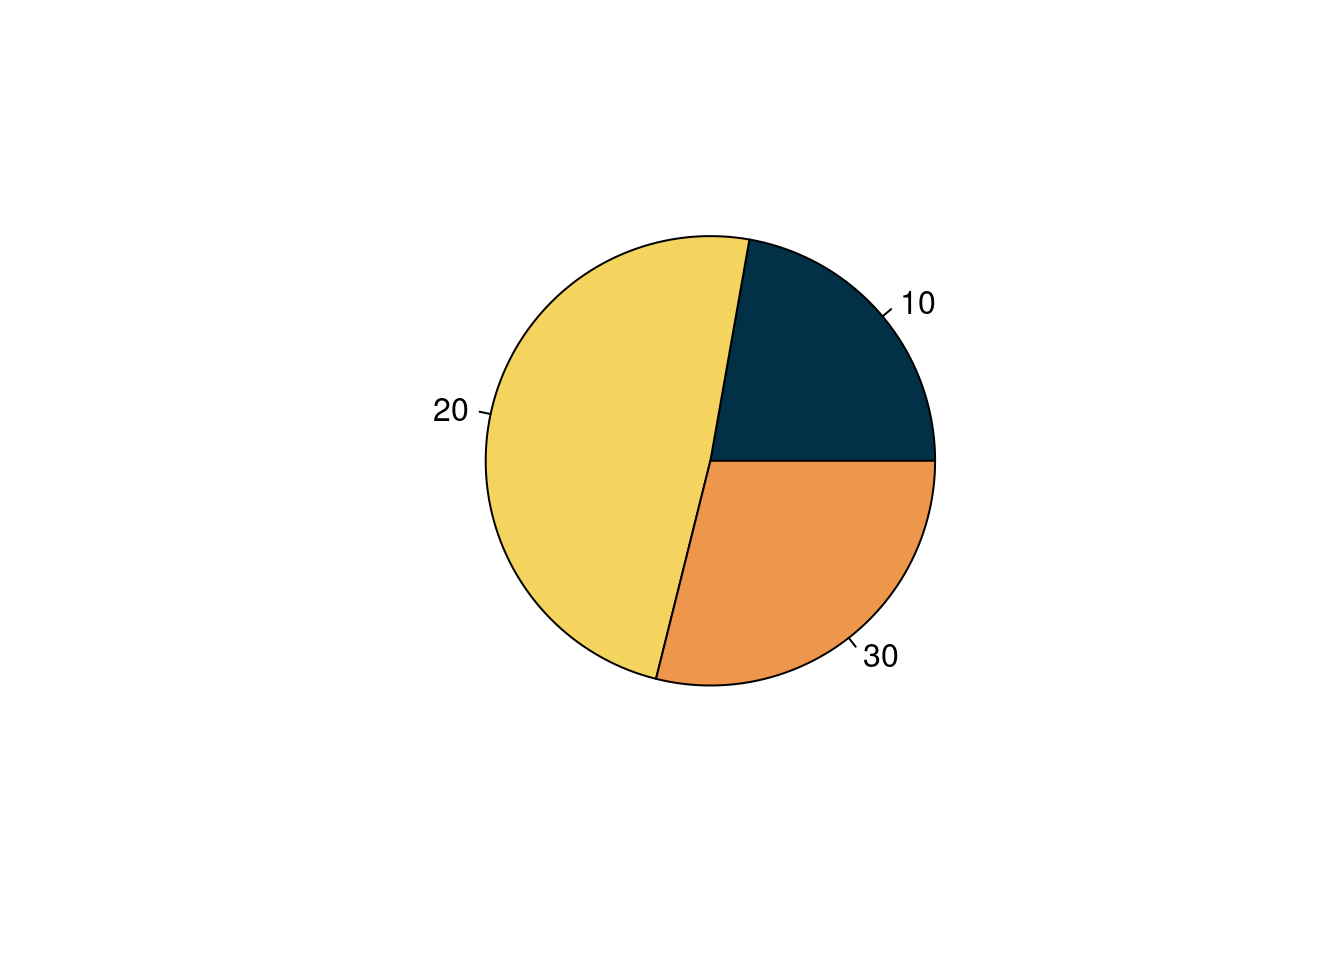
\includegraphics{Taller422_files/figure-latex/unnamed-chunk-1-1.pdf}

Suponga que el tiempo de secado se distribuye normal . Calcule un
intervalo de confianza para la diferencia de medias e interprete su
resultado

\begin{Shaded}
\begin{Highlighting}[]
\FunctionTok{var.test}\NormalTok{(A,B)}\SpecialCharTok{$}\NormalTok{conf.int}
\end{Highlighting}
\end{Shaded}

\begin{verbatim}
[1] 0.3588543 3.1837492
attr(,"conf.level")
[1] 0.95
\end{verbatim}

Como el IC para la razón de varianzas (0.3588543; 3.1837492) contienen a
1, asumimos que las varianzas son iguales

\begin{Shaded}
\begin{Highlighting}[]
\FunctionTok{t.test}\NormalTok{(A,B, }\AttributeTok{var.equal=}\NormalTok{T,}\AttributeTok{paired=}\NormalTok{F)}\SpecialCharTok{$}\NormalTok{conf.int}
\end{Highlighting}
\end{Shaded}

\begin{verbatim}
[1] -1.3922636 -0.8477364
attr(,"conf.level")
[1] 0.95
\end{verbatim}

Como el intervalo resultante es (-,-), indica que \(\mu_{A} < \mu_{B}\).
Por tal motivo se recomienda la compra de la marca A

\hypertarget{problema-4}{%
\section{\texorpdfstring{\textbf{Problema
4}}{Problema 4}}\label{problema-4}}

En una encuesta aleatoria realizada a 500 familias de la ciudad que
poseen televisión por cable, se encuentra que 340 tienen suscripción a
HBO. Calcule un intervalo de confianza para la proporción de familias
que tienen suscripción a HBO en la ciudad. Interprete el resultado
obtenido.

\hypertarget{problema-5}{%
\section{\texorpdfstring{\textbf{Problema
5}}{Problema 5}}\label{problema-5}}

Suponga que se desea realizar un estudio en la ciudad para estimar la
proporción de familias que tienen suscripción a HBO, con el fin de
repetir el estudio después de dos meses, de tal forma que permita
validar el efecto de publicidad de estos canales de televisión. Si se
requiere estimar una intervalo de confianza para la proporción con un
95\% de confianza y que la estimación de \(p\) este dentro de 0.02 del
valor verdadero, ¿Que tan grande debe ser la muestra?

\hypertarget{problema-6}{%
\section{\texorpdfstring{\textbf{Problema
6}}{Problema 6}}\label{problema-6}}

Se afirma que una persona podrá reducir su peso en un periodo de dos
semanas un promedio de 4.5 kilogramos con una nueva dieta. Los pesos de
7 mujeres de siguieron esta dieta se registraron antes y después de un
periodo de dos semanas.

\begin{Shaded}
\begin{Highlighting}[]
\NormalTok{pesant}\OtherTok{=}\FunctionTok{c}\NormalTok{(}\FloatTok{58.2}\NormalTok{, }\FloatTok{60.3}\NormalTok{, }\FloatTok{61.3}\NormalTok{, }\FloatTok{69.0}\NormalTok{, }\FloatTok{64.0}\NormalTok{, }\FloatTok{62.6}\NormalTok{, }\FloatTok{56.7}\NormalTok{)}
\NormalTok{pesdes}\OtherTok{=}\FunctionTok{c}\NormalTok{(}\FloatTok{60.0}\NormalTok{, }\FloatTok{54.9}\NormalTok{, }\FloatTok{58.1}\NormalTok{, }\FloatTok{62.1}\NormalTok{, }\FloatTok{58.5}\NormalTok{, }\FloatTok{59.9}\NormalTok{, }\FloatTok{54.4}\NormalTok{)}
\end{Highlighting}
\end{Shaded}

Pruebe la afirmacion sobrela dieta calculando un intervalo de confianza
del 95\% para la diferencia de medias . Suponga que las diferencias de
los pesos se distribuyen aproximadamente normal.

\hypertarget{problema-7}{%
\section{\texorpdfstring{\textbf{Problema
7}}{Problema 7}}\label{problema-7}}

El conjunto de datos de iris (de Fisher o Anderson) contiene las medidas
en centímetros de las variables longitud y ancho del sépalo y largo y
ancho del pétalo, respectivamente, para 50 flores de cada una de las 3
especies de iris : setosa, versicolor y virginica.

\begin{Shaded}
\begin{Highlighting}[]
\FunctionTok{data}\NormalTok{(iris)}
\FunctionTok{head}\NormalTok{(iris)}
\end{Highlighting}
\end{Shaded}

\begin{verbatim}
  Sepal.Length Sepal.Width Petal.Length Petal.Width Species
1          5.1         3.5          1.4         0.2  setosa
2          4.9         3.0          1.4         0.2  setosa
3          4.7         3.2          1.3         0.2  setosa
4          4.6         3.1          1.5         0.2  setosa
5          5.0         3.6          1.4         0.2  setosa
6          5.4         3.9          1.7         0.4  setosa
\end{verbatim}

Determine intervalos de confianza para cada una de las caracteristicas
por espacies. Existen diferencias entre los promedio del largo de los
sepalos de las especies setosa y virginica?

\hypertarget{problema-8}{%
\section{\texorpdfstring{\textbf{Problema
8}}{Problema 8}}\label{problema-8}}

Cuántos artículos deben incluirse en una muestra para estimar la
proporción de defectuosos con un error no mayor del 2\% y confiabilidad
del 95\%

\hypertarget{problema-9}{%
\section{\texorpdfstring{\textbf{Problema
9}}{Problema 9}}\label{problema-9}}

De 1000 casos seleccionados al azar de cáncer de pulmón, 823 resultaron
en la muerte dentro de los 10 años después de su detección. Construya un
intervalo de confianza para la tasa de mortalidad por cáncer de pulmón
del 95\%, de acuerdo con los datos suministrados. Interprete los
resultados obtenidos.

\hypertarget{problema-10}{%
\section{\texorpdfstring{\textbf{Problema
10}}{Problema 10}}\label{problema-10}}

A seis ingenieros que trabajan para el estado se les solicito realizar
un pronostico la tasa de inflación para el año entrante. La misma
petición se le realizo a ocho especialistas en finanzas que trabajan
para el sector privado. Los pronósticos entregado por los ingenieros son
los siguientes: 4.2 \%, 5.1 \%, 3.9 \%, 4.7 \%, 4.8 \%, 5.8 \%. Por su
parte los especialistas en finanzas pronosticaron: 5.7 \%, 6.1 \%, 5.2
\%, 4.9 \%, 4.6 \%, 4.5 \%, 5.2 \%, 5.5 \%. ¿Estan los especialistas
(ingenieros y financieros) realizando pronósticos similares? . Suponga
que los pronósticos realizados tienen distribucion normal. Construye un
intervalo de confianza para la diferencia de los promedios realizados
por los ingenieros y los especializadas en finanzas del 95\%. Concluya a
partir de los resultados.

\hypertarget{problema-11}{%
\section{\texorpdfstring{\textbf{Problema
11}}{Problema 11}}\label{problema-11}}

Los siguientes datos corresponden a las notas finales del curso de
matematicas fundamentales.

\begin{Shaded}
\begin{Highlighting}[]
\NormalTok{nf}\OtherTok{=}\FunctionTok{c}\NormalTok{(}\FloatTok{4.1}\NormalTok{, }\FloatTok{2.7}\NormalTok{, }\FloatTok{3.1}\NormalTok{, }\FloatTok{3.2}\NormalTok{, }\FloatTok{3.0}\NormalTok{, }\FloatTok{3.2}\NormalTok{, }\FloatTok{2.0}\NormalTok{, }\FloatTok{2.4}\NormalTok{, }\FloatTok{1.6}\NormalTok{, }\FloatTok{3.2}\NormalTok{, }\FloatTok{3.1}\NormalTok{, }\FloatTok{2.6}\NormalTok{, }\FloatTok{2.0}\NormalTok{, }\FloatTok{2.4}\NormalTok{, }\FloatTok{2.8}\NormalTok{, }
     \FloatTok{3.3}\NormalTok{, }\FloatTok{4.0}\NormalTok{, }\FloatTok{3.4}\NormalTok{, }\FloatTok{3.0}\NormalTok{, }\FloatTok{3.1}\NormalTok{, }\FloatTok{2.7}\NormalTok{, }\FloatTok{2.7}\NormalTok{, }\FloatTok{3.0}\NormalTok{, }\FloatTok{3.8}\NormalTok{, }\FloatTok{3.2}\NormalTok{, }\FloatTok{2.2}\NormalTok{, }\FloatTok{3.5}\NormalTok{, }\FloatTok{3.5}\NormalTok{, }\FloatTok{3.8}\NormalTok{, }\FloatTok{3.5}\NormalTok{, }
     \FloatTok{3.9}\NormalTok{, }\FloatTok{4.2}\NormalTok{, }\FloatTok{4.3}\NormalTok{, }\FloatTok{3.9}\NormalTok{, }\FloatTok{3.2}\NormalTok{, }\FloatTok{3.5}\NormalTok{, }\FloatTok{3.5}\NormalTok{, }\FloatTok{3.7}\NormalTok{, }\FloatTok{4.1}\NormalTok{, }\FloatTok{3.7}\NormalTok{, }\FloatTok{3.5}\NormalTok{, }\FloatTok{3.6}\NormalTok{, }\FloatTok{3.2}\NormalTok{, }\FloatTok{3.1}\NormalTok{, }\FloatTok{3.4}\NormalTok{, }
     \FloatTok{3.0}\NormalTok{, }\FloatTok{3.0}\NormalTok{, }\FloatTok{3.0}\NormalTok{, }\FloatTok{2.7}\NormalTok{, }\FloatTok{1.7}\NormalTok{, }\FloatTok{3.6}\NormalTok{, }\FloatTok{2.1}\NormalTok{, }\FloatTok{2.4}\NormalTok{, }\FloatTok{3.0}\NormalTok{, }\FloatTok{3.1}\NormalTok{, }\FloatTok{2.5}\NormalTok{, }\FloatTok{2.5}\NormalTok{, }\FloatTok{3.6}\NormalTok{, }\FloatTok{2.2}\NormalTok{, }\FloatTok{2.4}\NormalTok{, }
     \FloatTok{3.1}\NormalTok{, }\FloatTok{3.3}\NormalTok{, }\FloatTok{2.7}\NormalTok{, }\FloatTok{3.7}\NormalTok{, }\FloatTok{3.0}\NormalTok{, }\FloatTok{2.7}\NormalTok{, }\FloatTok{3.0}\NormalTok{, }\FloatTok{3.2}\NormalTok{, }\FloatTok{3.1}\NormalTok{, }\FloatTok{2.4}\NormalTok{, }\FloatTok{3.0}\NormalTok{, }\FloatTok{2.7}\NormalTok{, }\FloatTok{2.5}\NormalTok{, }\FloatTok{3.0}\NormalTok{, }\FloatTok{3.0}\NormalTok{, }
     \FloatTok{3.0}\NormalTok{, }\FloatTok{3.2}\NormalTok{, }\FloatTok{3.1}\NormalTok{, }\FloatTok{3.8}\NormalTok{, }\FloatTok{4.1}\NormalTok{, }\FloatTok{3.7}\NormalTok{, }\FloatTok{3.5}\NormalTok{, }\FloatTok{3.0}\NormalTok{, }\FloatTok{3.7}\NormalTok{, }\FloatTok{3.7}\NormalTok{, }\FloatTok{4.1}\NormalTok{, }\FloatTok{3.7}\NormalTok{, }\FloatTok{3.9}\NormalTok{, }\FloatTok{3.7}\NormalTok{, }\FloatTok{2.0}\NormalTok{)}
\end{Highlighting}
\end{Shaded}

Construya un intervalo del 95\% confianza para el promedio de la nota
final del curso de matematicas fundamentales. Interprete su resultado

\hypertarget{problema-12}{%
\section{\texorpdfstring{\textbf{Problema
12}}{Problema 12}}\label{problema-12}}

Una muestra de siete bloques de concreto tienen la siguiente fuerza de
compresión medida en MPa . Los resultados obtenidos son:

\begin{Shaded}
\begin{Highlighting}[]
\NormalTok{x}\OtherTok{=}\FunctionTok{c}\NormalTok{(}\FloatTok{1367.6}\NormalTok{, }\FloatTok{1411.5}\NormalTok{, }\FloatTok{1318.7}\NormalTok{, }\FloatTok{1193.6}\NormalTok{, }\FloatTok{1406.2}\NormalTok{, }\FloatTok{1425.7}\NormalTok{, }\FloatTok{1572.4}\NormalTok{)}
\end{Highlighting}
\end{Shaded}

Estime un intervalo de confianza del 95\% para la media de la fuerza de
compresion de los bloques de concreto

\hypertarget{problema-13}{%
\section{\texorpdfstring{\textbf{Problema
13}}{Problema 13}}\label{problema-13}}

Los directivos de una ensambladora de automóviles de gran tamaño están
tratando de decidir si compraran neumáticos de la marca A o de la marca
B para sus modelos nuevos. Con el fin de ayudarlos a tomar una decisión
se realiza un experimento en el que se usan 12 neumáticos de cada marca.
Los neumáticos se utilizan hasta que se desgastan completamente. Los
resultados son los siguientes:

\begin{Shaded}
\begin{Highlighting}[]
\NormalTok{A}\OtherTok{=}\FunctionTok{c}\NormalTok{(  }\DecValTok{55145}\NormalTok{, }\DecValTok{58026}\NormalTok{, }\DecValTok{58795}\NormalTok{, }\DecValTok{54660}\NormalTok{, }\DecValTok{61153}\NormalTok{, }\DecValTok{56969}\NormalTok{, }\DecValTok{61764}\NormalTok{, }\DecValTok{59094}\NormalTok{, }\DecValTok{60456}\NormalTok{, }\DecValTok{54557}\NormalTok{, }\DecValTok{52484}\NormalTok{, }\DecValTok{59600}\NormalTok{)}
\NormalTok{B}\OtherTok{=}\FunctionTok{c}\NormalTok{(}\DecValTok{60970}\NormalTok{, }\DecValTok{62409}\NormalTok{, }\DecValTok{60546}\NormalTok{, }\DecValTok{58508}\NormalTok{, }\DecValTok{58974}\NormalTok{, }\DecValTok{56682}\NormalTok{, }\DecValTok{59483}\NormalTok{, }\DecValTok{58048}\NormalTok{, }\DecValTok{73107}\NormalTok{, }\DecValTok{61977}\NormalTok{, }\DecValTok{55974}\NormalTok{, }\DecValTok{58522}\NormalTok{)}
\end{Highlighting}
\end{Shaded}

¿Que marca de neumáticos escogería entre las dos opciones de acuerdo a
la anterior informacion? Suponga que las poblaciones se distribuyen de
forma aproximadamente normal .

\hypertarget{problema-14}{%
\section{\texorpdfstring{\textbf{Problema
14}}{Problema 14}}\label{problema-14}}

El Director de una fabrica de muebles desea estimar el tiempo promedio
que toma perforar tres agujeros en una placa metálica que se utiliza en
la construcción de bases para mesas metálicas. El desea tener una
confianza del 95 \% para que la media muestral este dentro de 5 segundos
de la media real, suponiendo que \(\sigma=40\), obtenida en estudios
anteriores. Una de las firmas contactadas para la realización del
estudio indica que para esas condiciones, deberá realizar 175
mediciones. El Director le pide que revise la información suministrada y
le de su concepto.

\hypertarget{problema-15}{%
\section{\texorpdfstring{\textbf{Problema
15}}{Problema 15}}\label{problema-15}}

Un estudio realizado por MasterCard revelo que 131 de las 468 mujeres
que efectuaron compras en almacén lo hicieron utilizando la tarjeta de
crédito propia del almacén, mientras que 57 de 237 hombres utilizaron la
misma tarjeta para sus compras en el almacén. ¿ Existe evidencia
suficiente en los datos que permita concluir que la proporción de
mujeres es mayor que la proporción de hombres que utilizan la tarjeta de
crédito propia del almacén para realizar sus compras?

\hypertarget{cuxf3digo-r}{%
\section{\texorpdfstring{\textbf{Código
R}}{Código R}}\label{cuxf3digo-r}}

\begin{longtable}[]{@{}
  >{\centering\arraybackslash}p{(\columnwidth - 2\tabcolsep) * \real{0.2400}}
  >{\raggedright\arraybackslash}p{(\columnwidth - 2\tabcolsep) * \real{0.7600}}@{}}
\toprule()
\begin{minipage}[b]{\linewidth}\centering
parámetro
\end{minipage} & \begin{minipage}[b]{\linewidth}\raggedright
código R
\end{minipage} \\
\midrule()
\endhead
\(\mu\) & \texttt{t.test(x,\ coef.level=\ 1−a)\$conf.int} \\
\(p\) & \texttt{prop.test(x,n,\ conf.level=0.95)\$conf.int} \\
\(\mu_{1}-\mu_{2}\) &
\texttt{t.test(datos1,datos2,\ paired=T)\$conf.int} \\
& \texttt{t.test(datos1\ datos2,\ var.equal=T)\$conf.int} \\
& \texttt{t.test(datos1\ datos2,\ var.equal=F)\$conf.int} \\
\(p_{1} − p_{2}\) & \texttt{prop.test(c(x1,x2),\ c(n1,n2))\$conf.int} \\
\(\sigma^{2_{1}} / \sigma^{2}_{2}\) &
\texttt{var.test(datos1,\ datos2)\$conf.int} \\
\bottomrule()
\end{longtable}

\begin{longtable}[]{@{}
  >{\centering\arraybackslash}p{(\columnwidth - 2\tabcolsep) * \real{0.2400}}
  >{\raggedright\arraybackslash}p{(\columnwidth - 2\tabcolsep) * \real{0.7600}}@{}}
\toprule()
\endhead
& \texttt{install.packages("devtools")} \\
& \texttt{devtools::install\_github("dgonzalez80/paquetepye")} \\
& \texttt{library(paqueteDEG)} \\
& \textbf{tamaño de muestra} \\
\(\mu\) &
\texttt{paqueteDEG::sizemu(1.96,345,2)\ \ \ \ \ \#\ sizemu(z,sigma2,error)} \\
\(p\) &
\texttt{paqueteDEG::sizep(1.96,0.5,0.05)\ \ \ \#\ sizep(z,prob,error)} \\
\(n_{aj}\) &
\texttt{paqueteDEG::adjusted\_size(385,2000)\ \#\ adjusted\_size(n,N)} \\
\bottomrule()
\end{longtable}

\end{document}
